\documentclass{standalone}
\usepackage{pgfplots}
\begin{document}
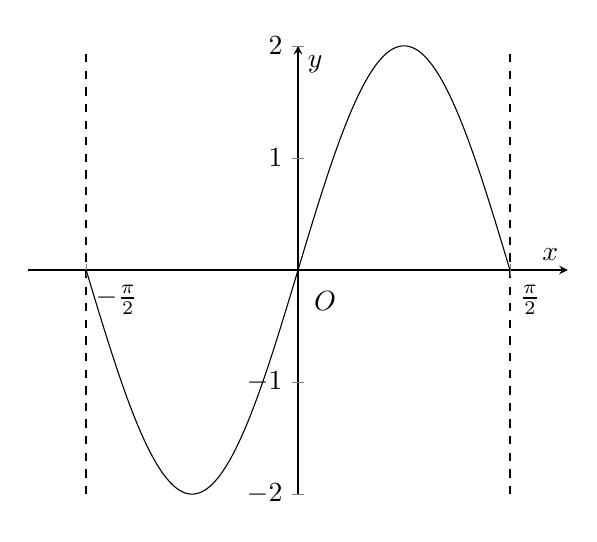
\begin{tikzpicture}
\begin{axis}
[
ymin=-2,ymax=2,
xmin=-2,xmax=2,
%clip=false,
xtick=\empty,
ytick=\empty,
extra x ticks={-1.5708, 1.5708},
extra x tick labels={$-\frac{\pi}{2}$, $\frac{\pi}{2}$},
extra y ticks={-2, -1, 1, 2, 3, 4},
extra y tick labels={$-2$, $-1$, $1$, $2$},
every extra x tick/.style={
    xticklabel style={anchor=north west},
    grid=major,
    major grid style={thick,dashed,black}
},
axis lines = center,
xlabel=$x$,ylabel=$y$,
domain=-0.5*pi:0.5*pi,
samples=200,
]
\addplot [black] {2*sin(deg(2*x))};
\node at (axis cs:0.2, -0.28) {$O$} ;
\end{axis}
\end{tikzpicture}
\end{document}
